
\chapter{Effect on Subnational Governmentals' Revenue Collection Behavior}

\section{Problem Introduction}

Once received transfer payment from national government, subnational government should react in terms of both spending and revenue collection behavior. Chapter 4 is about the reaction in spending. In this chapter, I'll discuss the effect of IGT on subnational's revenue collection. Specifically, I focus on the reaction in tax collection effort.

In most of the countries, administrative institution has no allowance to change the legal tax rate arbitrarily, while the intergovernmental transfer fluctuate frequently at a yearly base. For example, in America, it's senate and house of representatives' job to alter the legal tax rate. This discordance means administrative branch would change the tax collection effort to control the actual tax burden. Subnational governments has many methods to alter the actual tax burden without changing the legal tax rate such as tax deduction, tax relief etc. To summarize, in this chapter, the problem is to investigate subnational governments' reaction on tax collection effort by solving subnational governments' Ramsey problem.

\section{Former Theory and Bibliography}

Inherent to the nature of general transfer is that transfer would lead to tax fungibility effect, which means transfer would substitute local governments' revenue collection efforts. This phenomenon is also referred to as the crowding out effect on tax effort and has been supported by bunch of evidences \cite{inman1988federal,peterson1997decentralization,litvack1998rethinking}. Empirical evidence in both developed and developing countries has further confirmed this theoretical inference. For example, Nicholson \cite{nicholson2008fiscal} discovered the fungibility effect of intergovernmental transfer on tax effort at the state level in Germany and the United States. Similarly, Baretti \cite{2002A}, Aragon and Gayoso \cite{aragon2005intergovernmental}, Panda \cite{panda2009central}, Mogues \cite{mogues2012external}, and Bravo \cite{bravo2013income} found similar evidence in developing countries such as Peru, India, Ghana, and Chile. In short, the fungibility of intergovernmental transfer on tax revenue could lead to a decrease in the efforts of governments to collect tax revenue once they receive sufficient funds from transfer payments.

The fungibility effect seems natural when the range of study is constrained in one specific jurisdictions. Once multiple jurisdictions and horizontal competition are introduced into the consideration, one opposite impact also seems to be reasonable. Some theoretical research contend that the local jurisdictions should be motivated to lower the tax burden since they are facing the tax competition. The lower tax burden may attract capital, citizen or enterprise into the area, thus the local governments may actively give up the tax benefits they could have collected. In another word, the tax competition may encourage the local governments to expand the tax base rather than increase the tax effort. The revenue from intergovernmental transfer may neutralize this subjective intention, thus the tax effort would be positively affected. Bucovetsky and Smart \cite{2010The}, Buettner \cite{2006The} describe this guess in their analysis of fiscal equalization. Liu \cite{2011Intergovernmental}
found some empirical evidence in China. However, compared to the study on fungibility, the investigation on this effect are seldom systemically investigated in theoretical level, limited literature are empirical analysis.

To synthesize the literature, two potential gaps arise. Firstly, akin to the research on the impact of intergovernmental transfers on local governments' spending preferences, the focus of  is mainly on general transfers, with little emphasis on categorical transfers. Even in some literatures that try to discuss the effect of strings attached on the grants and points out the potential effect of the strings, they do not conduct a rigorous theoretical discussion, thus they got different conclusions \cite{gramlich1997intergovernmental,chubb1985political,nicholson2004goal}. Nicholson \cite{nicholson2008fiscal} did a fixed regression and assert that the general grants-in-aid exert downward pressure on state tax effort. Dash and Raja \cite{dash2013intergovernmental}get opposite evidence and find stimulative effect on tax collect efficiency.

The second issue is that most of the literature in investigating the effect of grants with restriction are theoretical conjecture rather than empirical investigation. Empirical evidence is surprisingly limited. Brunt and Khdari's \cite{2016The} research on the effect of categorical grants in Morocco failed to yield a conclusive result, which they attribute to political influence, leaving ample room for local governments to negotiate.

To address the identified gaps in the literature, I set up a one-period Ramsey problem in this study to analyze the tax collection behavior of subnational governments when received categorical transfer.  To further validate the theoretical inferences, empirical investigation was conducted in Chapter 6. Compared to the research in this area, my investigation get implication on both general transfer and categorical transfer. The utilization of both qualitative and quantitative methods in this study allowed for a solid understanding of the research topic.
% I get the access to understand how central and subnational governments get to the equilibrium condition rather than just assume the equilibrium condition. Another potential issue for the theory construction is that the analysis is on a macro base, for example, most of the literature set governments as player and the goal of governments is to maximize the fiscal revenue by default. However, governments is an organization rather than a person, and this default setting on macro level doesn't explain why this organization wants to maximize the revenue.By adding the personal politicians' preference components into the utility function in game theory analysis, we can understand the fiscal behavior on a more micro base. And I combine the game theory analysis result with the prototypical benchmark model in section 3.1.1 to connect both spending side (lower left side of Figure \ref{Figure 3.1}) and revenue side (lower right side of Figure \ref{Figure 3.1}).

\section{A Ramsey Problem for Subnational Government}
The Ramsey problem for subnational government is to maximize the utility under specific budget constraint, thus the model is constructed from budget constraint aspect and utility aspect.

\subsection{Budget Constraint for Subnational Government}

The budget of subnational government comes from two parts---transfer from national government and tax collection. To address the underemphasized categorical transfer, I assume national government make both general transfer and categorical transfer to subnational government.

I follow the setting in Chapter 2 on general transfer that general transfer to region $i$ is related to the total output in $i$, which I represents as $F_i$. The allocation function for general transfer amount is $T_0-\sigma F_i$, where $T_0$ is the benchmark amount when the tax base in $i$ is 0 and $\sigma$ is the "equalization parameter". A greater $\sigma$ typically means national government prefer to a equalized development in different regions\footnote{One this to notice, in this chapter, the amount of general transfer and categorical transfer is exogenous for subnational government.}.

In terms of categorical transfer, I still follow the matching mechanism in Chapter 2. The national government can decide the categorical transfer be spent either on productive public goods $P$ or welfare public goods $W$. Besides, the matching ration in different sectors $0<m<1$ and $0<n<1$ are also decided by national government, thus the transfer flow direction and matching ration is also exogenous for subnational government. In this logic, the total amount of categorical transfer can be written as:

\begin{equation}
    m_iP_i+n_iE_i
\end{equation}

Revenue source of the subnational government comes from intergovernmental transfer, including general transfer and categorical transfer, and tax revenue. Total revenue is spent on either productive public goods or welfare-oriented public goods, thus the budget constraint for subnational government is:
\begin{equation}
    p_i + w_i = \tau_i F_i + (T^0 - \sigma F_i) + (m p_i + n w_i)
\end{equation}

\subsection{Utility Construction}

I assume there is a representative company and the production function in region $i$ is:

\begin{equation}
    F_i=A_iK_i^{\alpha}P_i^{\beta} \label{F}
\end{equation}

where $K$ is the capital amount and $P$ is the productive,  $\alpha$ and $\beta$ is the elasticity of $K$ and $P$. I assume that $\alpha+\beta<1$, since the the capital and productive spending are marginal decline.

Subnational government care about both welfare utility and after tax output, thus the utility function for subnational government can be expressed as:

\begin{equation}
    U_i = (1 - \tau_i) F_i + \lambda_iW_i \label{U}
\end{equation}
where $\tau_i$ is actual tax rate, which may affected by government's subjective collection willing and ability. The $\lambda_i$ is the demand of welfare utility. A greater $\lambda_i$ means subnational government prefer welfare utility and make light of productive utility, vice versa.


\end{itemize}

\section{Model Inference}

Based on the construction I set above, the subnational government solve the Ramsey problem. The total revenue is spent on either $P_i$ and $W_i$. The budget constraint can be list as:
\begin{equation}
    P_i+W_i=\tau_iF_i+T_i \label{1}
\end{equation}

where $T_i$ is the total amount of transfer payment, which equals to

\begin{equation}
    (T^0 - \sigma F_i) + (m p_i + n w_i)\label{2}
\end{equation}

Under the assumption of free capital flow, the economic competition would lead to a final equilibrium and achieve same capital return. The equilibrium condition is
\begin{equation}
    (1-\tau_i)\frac{\partial F_i}{K_i}=r\label{R}
\end{equation}
where $r$ is capital return. With equation \ref{F} and \ref{R}, I can express capital as a function of $P,r$ and $A_i$
\begin{equation}
    K_i(P_i,r,A_i)=[\frac{1}{r}(1-\tau_i)A_i\alpha P_i^\beta]^\frac{1}{1-\alpha}\label{K}
\end{equation}
For given $r$, subnational government choose $P_i$ to maximize the utility, thus I have:

\begin{equation}
    \frac{\partial F_i}{\partial P_i} + \frac{\partial F_i}{\partial K_i} \frac{\partial K_i}{\partial P_i} = \frac{\lambda_i\left(1-m_i\right)}{\left(1-\tau_i\right)\left(1-n_i\right)+\lambda_i\left(\tau_i-\sigma_i\right)}\label{P}
\end{equation}
which means the marginal utility for productive goods should equals to the marginal cost. With equation \ref{F},\ref{K},\ref{P}, the optimal amount of $P$ can be expressed as function:

\begin{equation}
    P_i= \left\{r^{-\alpha} A_i \alpha^\alpha(1-\alpha)^{\alpha-1} \beta^{1-\alpha}\left(1-\tau_i\right)^\alpha\left[\frac{\left(1-\tau_i\right)\left(1-n_i\right)+\lambda_i\left(\tau_i-G_i\right)}{\lambda_i\left(1-m_i\right)}\right]^{1-\alpha}\right\}^{\frac{1}{1-\alpha-\beta}} \label{PP}
\end{equation}

Plug equation \ref{PP} into equation \ref{F}, the output in region $i$ $F_i$ can be represented as function:
\begin{equation}
    F_i=A_i^{\frac{1}{1-\alpha-\beta}}\left(\frac{1-\tau_i}{r}\right)^{\frac{\alpha}{1-\alpha-\beta}}\left(\frac{\beta}{1-\alpha}\right)^{\frac{\beta}{1-\alpha-\beta}}\alpha^{\frac{\alpha}{1-\alpha-\beta}}\left[\frac{\left(1-\tau_i\right)\left(1-n_i\right)+\lambda_i\left(\tau_i-\sigma_i\right)}{\lambda_i\left(1-m_i\right)}\right]^{\frac{\beta}{1-\alpha-\beta}} \label{FF}
\end{equation}
Combined with equation \ref{1} and \ref{2}, the welfare oriented spending in region $i$ is:

\begin{equation}
    W_i=\frac{[(\tau_i-\sigma_i)F_i-(1-m_i)P_i+T^0]}{1-n_i}
\end{equation}\label{W}

Based on equation \ref{U},\ref{PP},\ref{FF} and \ref{W}, the utility for subnational government is:
\begin{equation}
    U_i=A_i^\theta \frac{\alpha^{\alpha \theta} \beta^{\beta \theta}}{\theta(1-\alpha)^{(1-\alpha) \theta} r^{\alpha \theta}}\frac{\left(1-\tau_i\right)^{\alpha \theta}\left[\left(1-\tau_i\right)\left(1-n_i\right)+\lambda_i\left(\tau_i-\sigma_i\right)\right]^{(1-\alpha) \theta}}{\left[\lambda_i\left(1-m_i\right)\right]^{\beta \theta}\left(1-n_i\right)} + \frac{\lambda_iT^0}{1-n_i} \label{UU}
\end{equation}
where $\theta=\frac{1}{1-\alpha-\beta}$.

The question I want to make suggestion on is the effect of transfer payment on the actual tax collection efficiency. From equation \ref{UU}, one obvious implication is that both parameters in general transfer and categorical transfer is affecting actual tax efficiency. With equation \ref{UU}, we can shed light on $\frac{d \tau_i}{d\sigma_i}$,$\frac{d \tau_i}{m_i}$ and $\frac{d \tau_i}{n_i}$.

\section{Affecting Mechanism}
I'll start with the affecting mechanism of general transfer. From equation \ref{UU}, changing of $\sigma_i$ would change $\tau$. Solved by implicit function theorem, I have:

\begin{equation}
    \frac{d \tau_i}{d \sigma_i}=-\frac{\lambda_i}{\frac{\alpha}{1-\alpha} \frac{\left(1-\tau_i\right)\left(1-n_i\right)+\lambda_i\left(\tau_i-\sigma_i\right)}{1-\tau_i}+\left(1-n_i-\lambda_i\right)} \label{gone}
\end{equation}

From equation \ref{FF}, $\frac{\partial F_i}{P_i}+\frac{\partial F_i}{K_i}\frac{\partial K_i}{\partial P_i}>0$, thus I have $(1-\tau_i)(1-n_i)+\lambda_i(\tau_i-\sigma_i)>0$. This means equation \ref{gone} gives two implications:
\begin{itemize}
    \item When $n_i+\lambda_i \leq 1$, $\frac{d \tau_i}{d \sigma_i}<0$
    \item When $n_i+\lambda_i>1+\frac{\alpha \lambda_i(1-\sigma_i)}{1-\tau_i}$,$\frac{d \tau_i}{d \sigma_i}>0$
\end{itemize}

A greater $n_i$ means national government concentrate on the welfare spending and a greater $\lambda_i$ means local government care more about welfare effect. Based on these two implications, we have proposition 11.

\textbf{Proposition 11: When both national and subnational government care more about productive utility, more general transfer would make subnational government lower down actual efficiency, vice versa.}

The explain is, when both levels government care more about productive utility, local government would treat general transfer as a free subsidy. A lower actual tax burden would stimulate capital inflow and boost the economy output. In this circumstance, the tax fungibility effect is in the dominate position. However when both levels of government cares more about welfare utility, the tax competition effect would be weaken. In this condition, the general transfer would lead to a greater actual tax burden $\tau_i$. Besides, when we say care more or care less, 1 and $1+\frac{\alpha \lambda_i(1-\sigma_i)}{1-\tau_i}$ working as the threshold.



Proposition 11 is about the effect of general transfer on actual tax rate. From equation \ref{UU}, we can also got some implication on the effect of categorical transfer. The effect of productive matching ration can be calculated as:

\begin{equation}
    \frac{d \tau_i}{d m_i}=\frac{\beta(1-m_i)^{-1}}{\alpha \frac{\left(1-\tau_i\right)\left(1-n_i\right)+\lambda_i\left(\tau_i-\sigma_i\right)}{1-\tau_i}+(1-\alpha)(1-\lambda_i-n_i)} \label{mone}
\end{equation}

Since $0<m<1$, whether equation \ref{mone} is positive or not is decided by denominator. Similarly, 1 and $1+\frac{\alpha \lambda_i(1-\sigma_i)}{1-\tau_i}$ also act as two thresholds. From the calculation, we have:
\begin{itemize}
    \item When $n_i+\lambda_i\leq 1$, $\frac{d \tau_i}{d m_i}>0$
    \item When $1<n_i+\lambda_i<1+\frac{\alpha \lambda_i(1-\sigma_i)}{1-\tau_i}$, $\frac{d \tau_i}{d m_i}>0$
    \item When $n_i+\lambda_i>1+\frac{\alpha \lambda_i(1-\sigma_i)}{1-\tau_i}$,$\frac{d \tau_i}{d m_i}<0$
\end{itemize}

Thus I have proposition 12.

\textbf{Proposition 12: When both national and subnational governments care more about productive spending, more categorical transfer on productive public goods would stimulate a higher actual tax rate, vice versa.}

The potential explain is: higher taxation income can both restrain and stimulate economy output when subnational government care more on productive utility, since more spending on $P$ is also a fiscal stimulus for $F_i$. In the condition with no transfer, subnational governments would control the $\tau_i$ such that marginal suppression effect equals marginal stimulate effect such as the peak of Laffer Curve\cite{laffer2004laffer}. When national government make categorical transfer directed to $P$, tax collection would stimulate the economy output since marginal stimulate effect would surpass marginal suppression effect. For subnational governments preferring productive utility, this would lead them to collect more tax and invest into the productive spending. However if subnational governments care more about welfare public goods, categorical transfer on $P$ would not encourage subnational governments to collect more tax.

Except for the effect of categorical transfer on productive public goods, transfer on welfare public goods may also affect subnational governments' tax collection. The marginal effect of $n_i$ can be calculated by implicit function theorem and envelop theorem as:
\begin{equation}
    \frac{d \tau_i}{n_i}=\frac{\left(1-n_i\right)^{-1}\left[-\beta \theta\left(1-\tau_i\right)\left(1-n_i\right)-\lambda\left(\tau_i-\sigma_i\right)\right]}{\alpha \theta \frac{\left(1-\tau_i\right)\left(1-n_i\right)+\lambda_i\left(\tau_i-\sigma_i\right)}{1-\tau_i}+\theta(1-\alpha)\left(1-\lambda_i-n_i\right)} \label{none}
\end{equation}

The sign of equation \ref{none} is undecided however. Unlike equatin \ref{gone} and \ref{mone}, we cannot get a clear distinction about the sign of $\frac{d \tau_i}{n_i}$. This means the understanding of the welfare categorical transfer on tax collection is unclear.


% An empirical investigation is conducted to support the theoretical inference got by solving subnational government's Ramsey problem.

% In the average state, the state government funds approximately 50\%-70\% of roadway operation, maintenance and construction through gas tax, license revenues and bonds. The federal government typically provides about 20\%-30\% of state transportation revenues through grants administered by the Federal Highway Administration. The small remaining percentage of expenditures comes from a variety of other sources including local contributions, charges for services and investment income \cite{nicholson2011claiming}.
% \begin{figure}[H]
%     \centering
%     \subfigure[]{
%         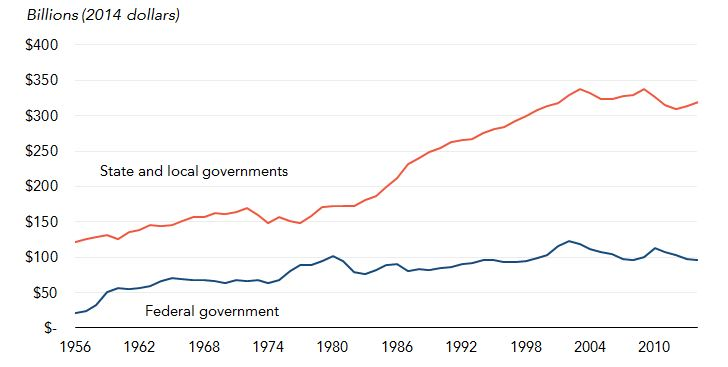
\includegraphics[width=0.8\textwidth]{Chapter-5/Figures/public spending on infrustracture.JPG}}
%     \subfigure[]{
%         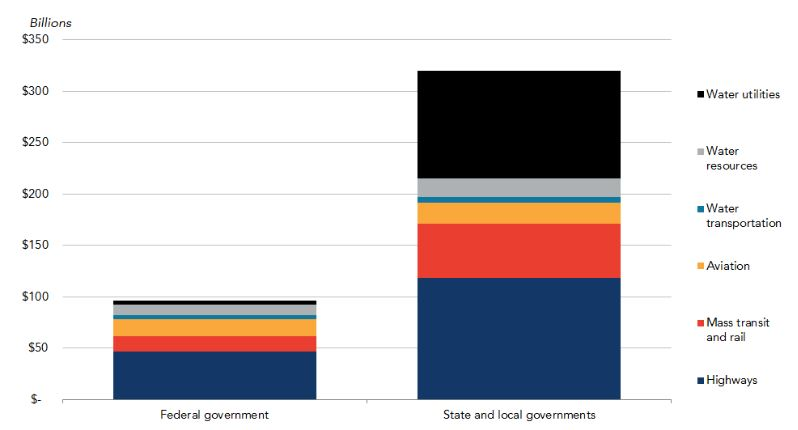
\includegraphics[width=0.8\textwidth]{Chapter-5/Figures/spending on infrastructure.JPG}}
%     \caption{Spending of Federal and Subnational Governments on Infrastructure}
%     \label{spendingonins}
% \end{figure}


% \begin{figure}[H]
%     \centering
%     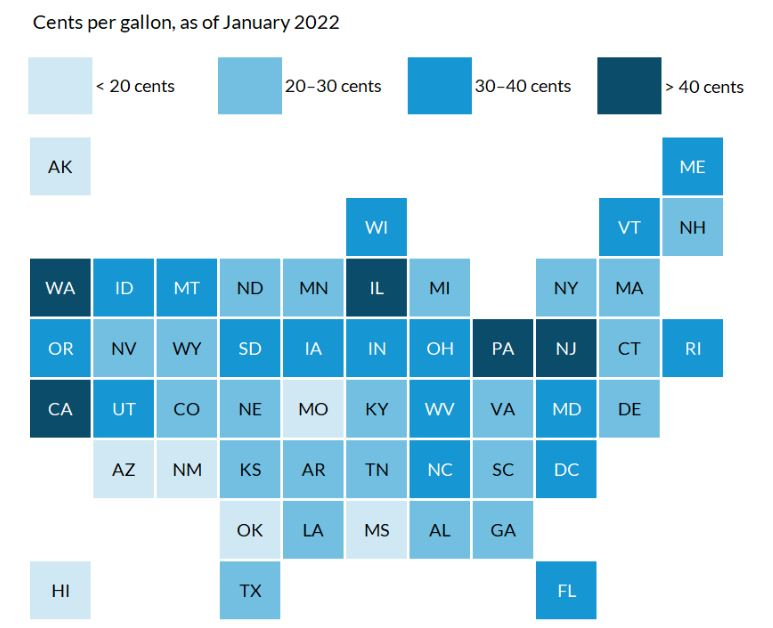
\includegraphics[scale=0.6]{Chapter-5/Figures/fuel tax2.JPG}
%     \caption{Gasoline Tax Rate on State Level
%         \texttt{} }
%     \label{gastax}
% \end{figure}

\section{Review and Summary}

Through a theoretical analysis, this chapter shed light on how intergovernmental transfer affects subnational governments' tax collection behavior. Compared to former investigation on related topics, this chapter add categorical transfer and different spending preferences into the Ramsey model.

Further review and modification is also necessary though. For example, the utility function is set as a compound of a Cobb-Douglas form and a linear form to get some arithmetic expression (such as the value of threshold, etc). This setting may not reflect the true tradeoff in real world. However this is a necessary compromise.